See Fig. \ref{fig:3.6.5_qten}.	In a parallelogram, the diagonals bisect each other. Hence
	\begin{align}
		\frac{\vec{A}+\vec{C}}{2} &= \frac{\vec{B}+\vec{D}}{2}
		\\
\therefore \frac{1+x}{2} = \frac{7}{2}, \frac{8}{2} &= \frac{y+5}{2} \\
\implies x=6,y&=3
\end{align}
	The following python code computes the value of x and y used in Fig. \ref{fig:3.6.5_qten}.
	\begin{lstlisting}
	./solutions/5/codes/lines/q10.py
	\end{lstlisting}
	\begin{figure}[!ht]
	\centering
	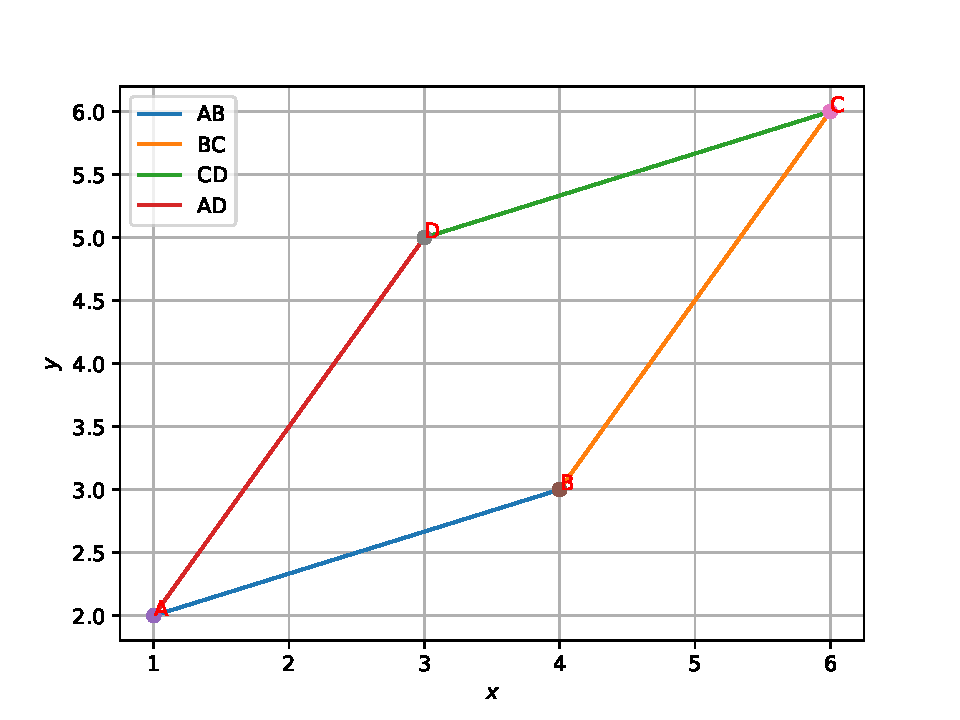
\includegraphics[width=\columnwidth]{./solutions/5/figs/lines/q10.eps}
	\caption{Parallelogram of Q.3.6.5}
	\label{fig:3.6.5_qten}	
	\end{figure}
	
		
